\documentclass{extarticle}
\usepackage{geometry}
\usepackage{graphicx}
\geometry{
 a4paper,
 total={170mm,257mm},
 left=20mm,
 top=20mm,
}

\title{Numdiag Questionnaire - Cahier des charges}
\author{Max Chateau}
\date{} 

\begin{document}
\maketitle{}
\section{Présentation du projet}
\subsection{Motivation}
Création d'une application pour créer et éditer des questionnaire à l'aide d'une interface utilisateur.
L'administrateur pourra ainsi éditer des questionnaire qui seront soit publiés sous forme de questionnaire unitaires pour des démos, soit utilisés pour les audits de l'application PUMA.\\
Les questionnaires seront à destination d'utilisateurs, qui lorsqu'ils auront terminé de le remplir, obtiendront un score en fonction des réponses données, ainsi que des recommandations basées sur le score global et/ou sur certaines réponses de questions.

\subsection{Principe}
\begin{itemize}
	\item Création de questions avec differents types de reponses (QCM, entiers, reéponses libres), avec un coéfficient qui affectera le score global en fonction de la réponse.
	\item Les questions seront regroupées dans une section, et ces sections composeront un questionnaire.
	\item Les questions peuvent avoir des dépendances avec des réponses (\textit{ie :} une réponse pourra conditionner l'affichage ou non d'une question)
\end{itemize}

\section{Détails techniques}
\subsection{Modèle de données}
\begin{figure}[h]
    \centering
    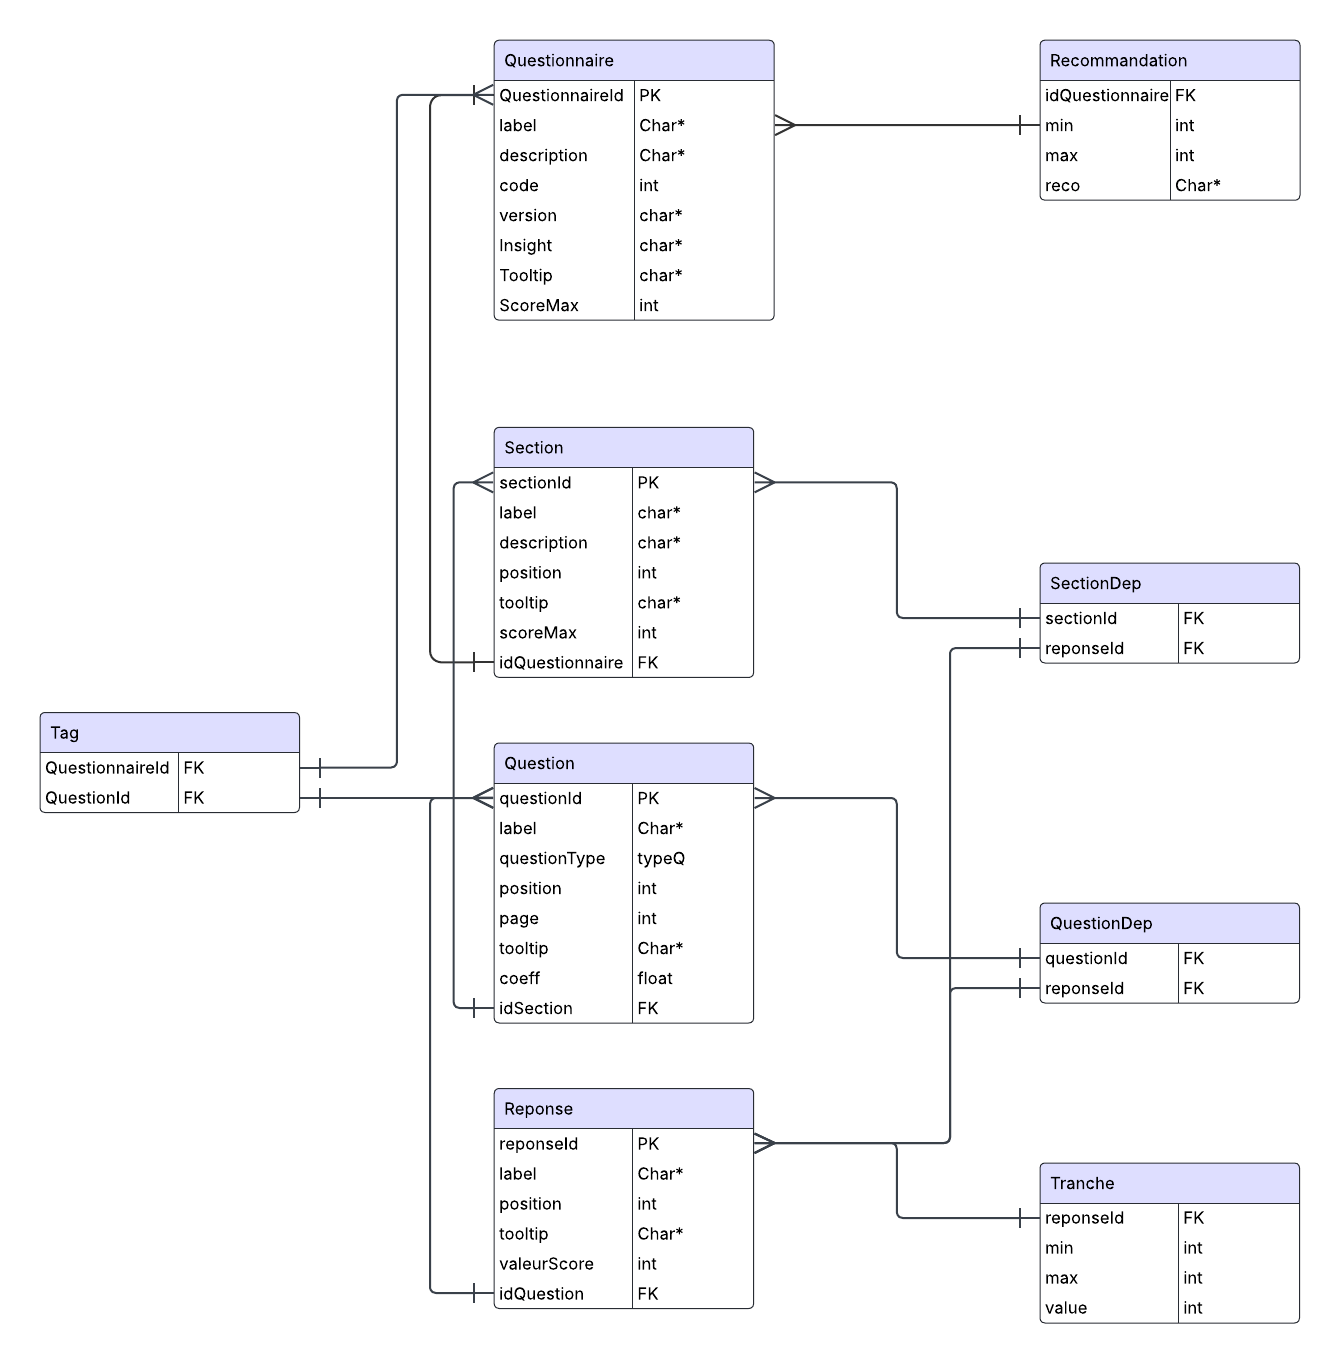
\includegraphics[width=0.5\textwidth]{NumdiagQuestionnaire.png}
    \caption{Modele Relationnel de Donnees}
    \label{fig:MRD}
\end{figure}

\subsection{Technos Utilisées}
Pour le front on va utiliser ReactJS + Vite.
Pour le back on utilisera ExpressJS. La base de données sera hebergée sur PostgreSQL.

Ces 3 services seront separés, et dockerisé, qui permettra d'utiliser docker-compose. 
On utilisera un unique repo Github pour ces 3 services.

\subsection{Fonctionnement Global}
La page admin affichera les differents questionnaires deja crees, il y aura la possibilite d'en creer des nouveaux, de les supprimer, de les modifier ou de les dupliquer.

\begin{figure}[h]
    \centering
    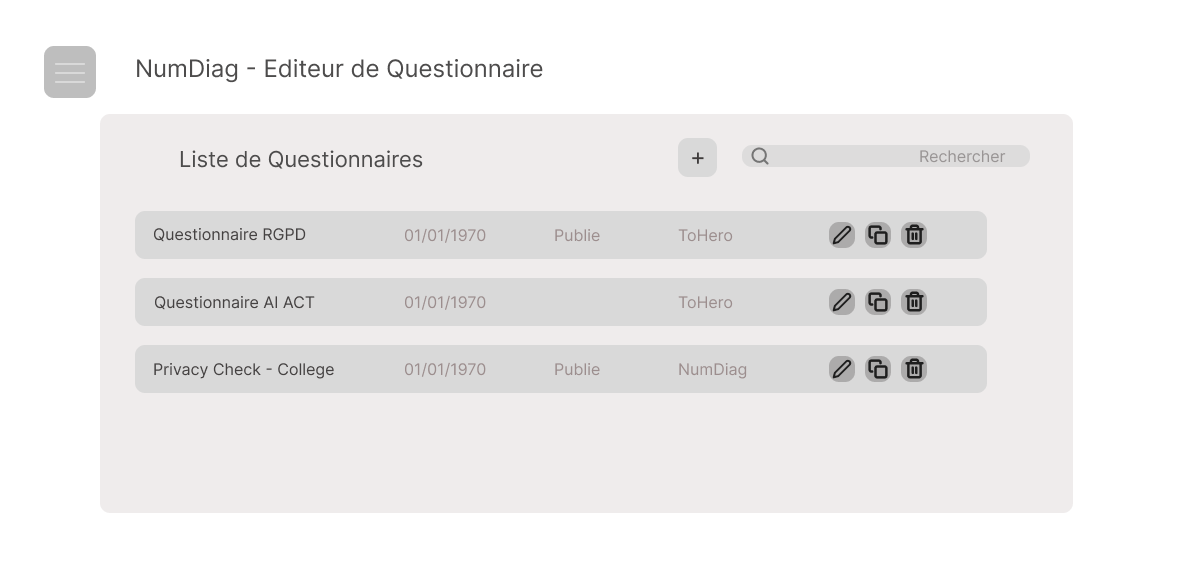
\includegraphics[width=0.8\textwidth]{adminVue.png}
    \caption{Page d'acceuil des questionnaires}
    \label{fig:AdminQuestionnaire}
\end{figure}

Lors de la modification d'un questionnaire, une nouvelle page s'ouvre pour afficher les sections, ainsi que les questions contenues dans chaque sections. On peut egalement afficher les differentes caracteristiques de la section pour les modifier.

\begin{figure}[h]
    \centering
    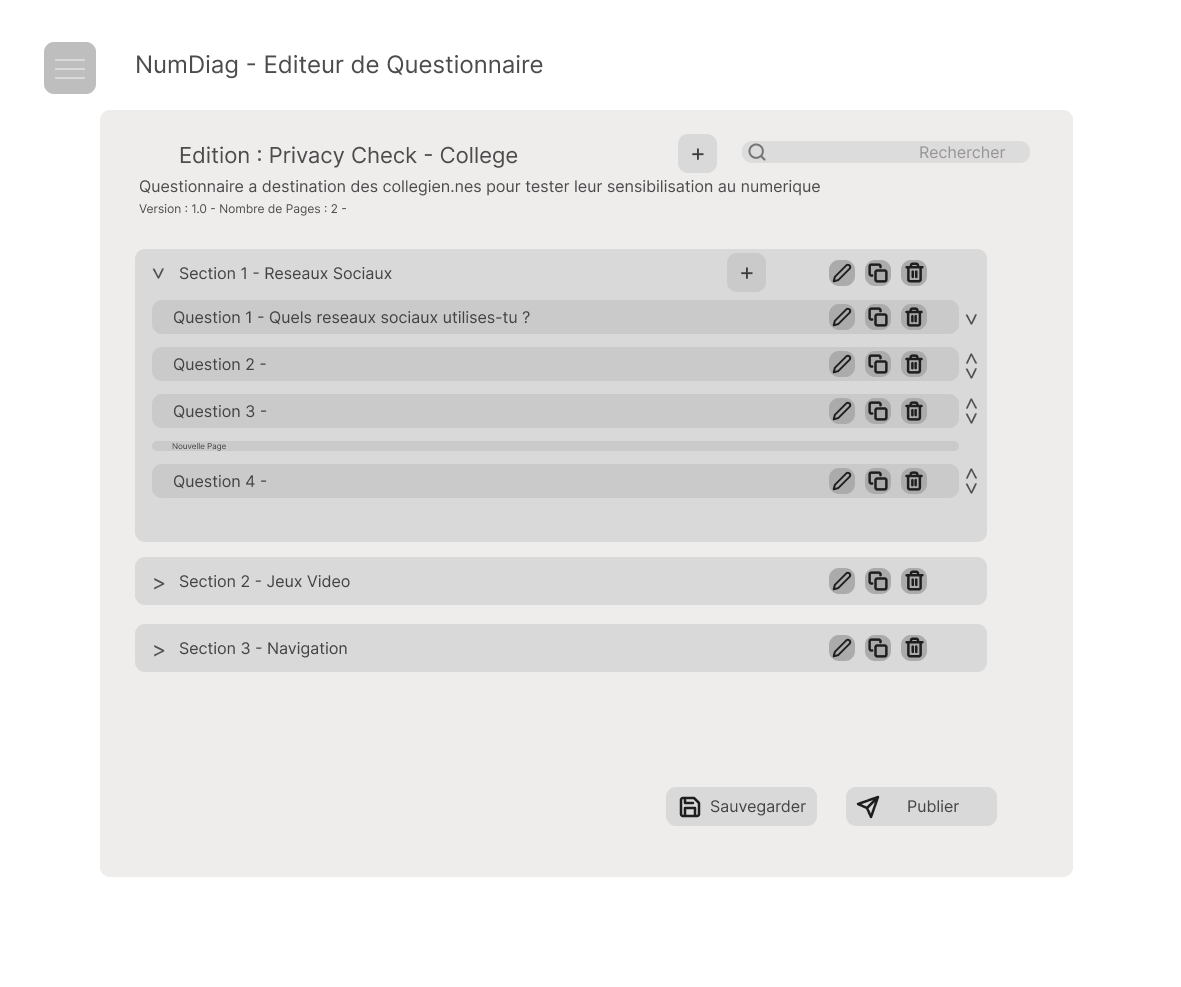
\includegraphics[width=0.7\textwidth]{questionnaireVue.png}
    \caption{Vue de modification d'un questionnaire}
    \label{fig:EditQuestionnaire}
\end{figure}

L'edition d'une question vient se faire dans une pop-up qui va demander les differentes informations qui sont les reponses, le score, les indications.

\begin{figure}[h]
    \centering
    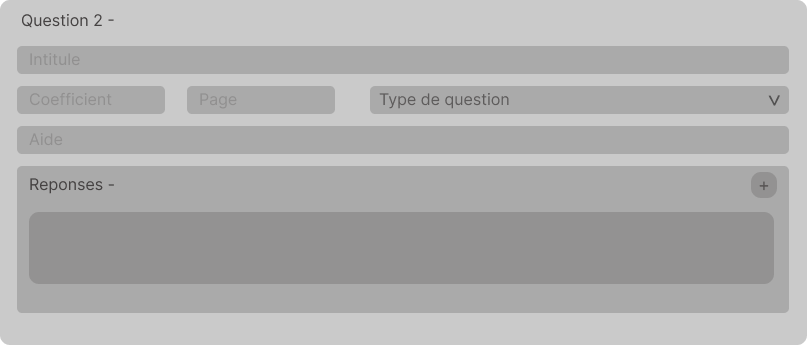
\includegraphics[width=0.8\textwidth]{questionVue.png}
    \caption{Vue de modification d'une question}
    \label{fig:EditQuestionnaire}
\end{figure}

\subsection{Fonctionnement Technique}
Une creation va envoyer les informations au back afin de verifier s'il est possible de creer l'element demande.\\
Lors d'une demande d'edition, le serveur va recuperer les toutes les informations du questionnaire associe demande dans la database, et les stocker en tampon, puis les envoyer a l'admin.\\
L'admin va faire les modifications de son cote, puis les envoyer au serveur, il va alors comparer avec ce qu'il a de son cote pour verifier si la modification est possible.\\
Quand l'admin a termine toutes les operations, le serveur va envoyer toutes les modifications dans la database.

Aucun element de la base de donnees ne sera fait directement dans le front, le serveur back fera office d'intermediaire pour transmettre les infos

\subsection{Les routes}
Les infos relatives aux differents appels API seront stockes dans le body des requetes\\
On implementera une architecture CRUD et REST pour toutes les routes de l'application\\
\underline{Les routes GET :}
\begin{itemize}
    \item url/questionnaire : renvoie les questionnaires avec toutes les infos ()
    \item url/questionnaire/:idquestionnaire : renvoie les les infos d'un questionnaire specifique
    \item url/questionnaire/:idquestionnaire/section : renvoie toutes infos de toutes les section d'un questionnaire 
\end{itemize}
\underline{Les routes POST :}
\begin{itemize}
    \item url/login : Permet a l'utilisateur de se connecter (mail + password)
    \item url/register : Permet a l'utilisateur de s'enrgistrer (mail + password + ...)
    \item url/questionnaire : Permet de creer un questionnaire (toutes les infos indiquees dans la database)
    \item url/questionnaire/:idquestionnaire/section : Permet de rajouter une section a unn questionnaire
    \item url/questionnaire/:idquestionnaire/section/:idsection/question : Une question a une section d'un questionnaire
    \item url/questionnaire/:idquestionnaire/section/:idsection/question/:idquestion/reponse : Permet de rajouter une reponse a une question

    \item url/document : creer un nouveau document
    \item url/document/:idDocument : permet d'editer un document (tag associe, description, etc...)

    \item url/createTag : permet de creer un tag
    \item url/linkTag : permet de lier un tag a une question
\end{itemize}
\end{document}